\chapter{Results}
\label{results}

In this section I present the results obtained while training word2doc repeatedly on different, random samples consisting of 1\% of
the full Wikipedia corpus (58,170 documents). Despite serious effort I was unable to train on a GPU and the largest subset I could
train on a CPU in a feasible time was about 1\%. Thus, I created ten random samples consisting of 1\% of the full dataset and
evaluated each. I now present my results averaged across all ten different samples. These results are compared to Facebook's document
retriever from DrQA \citep{drqa}. It should be noted that Facebook's document retriever has access to the full Wikipedia dataset while
word2doc only has access to 1\% of the Wikipedia corpus. Keep that in mind while reviewing these results.

As already mentioned in section \ref{exp:eval}, I use accuracy and mean average precision (MAP) to compare Facebook's document
retriever to word2doc. I compare both systems using all components (Full, Normal, Numbers, Typos, Abbreviations from Figure
\ref{fig:dataset-comp}) of the W2D-VD-400 evaluation dataset.

\section{Performance measured through Accuracy}

As mentioned above, all accuracies calculated for the 1\% dataset are averaged over ten different 1\% samples. This should
alleviate the randomness factor to a certain degree, and give more reliable data than just a single 1\% sample. All accuracies in
this section are computed using the full W2D-VD-400 test-set as evaluation data.

In order to measure accuracy more effectively, I chose four different testing criteria. First, I compare the performance of both
systems on the training set. This gives an indication of how well word2doc was trained and the potential of the document
retriever. Then I compare accuracies across only the single best document, the top five and the top ten retrieved documents.
This means if the target document is contained in the top one, top five or top ten returned documents, then the test case counts
as a success, otherwise it counts as a fail.

As can been seen in Figure \ref{fig:w2d-results-acc}, word2doc with 1\% of training data reached a training accuracy of 0.94\%.
Because all smaller samples that I trained eventually always reached a training accuracy of 0.999\%, it suggests that the model
is not fully trained
after 30 iterations. That is why in this case I also included accuracies for much smaller training sample, consisting of only 5000
randomly chosen documents (the baseline from Figure \ref{fig:w2d-model-tests}). The smaller dataset possibly hints at the full
potential if the 1\% dataset had been trained to a training accuracy of close to 100\%.

\begin{figure}
  \begin{center}
    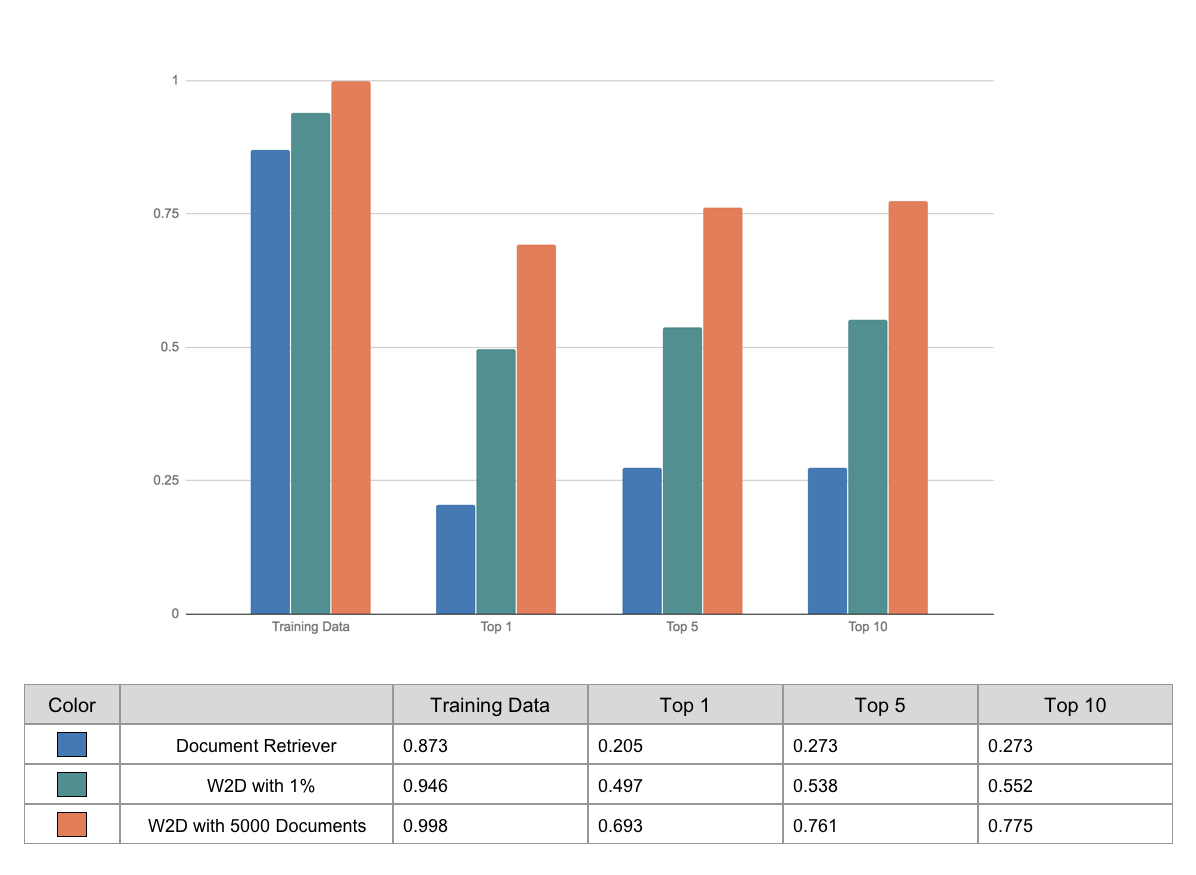
\includegraphics[scale=0.28]{w2d-results-acc.png}
  \end{center}
  \captionsetup{width=.75\linewidth}
  \caption{Facebook's document retriever vs. Word2doc Performance [Accuracies] with the full W2D-VD-400 used as evaluation data.}
  \label{fig:w2d-results-acc}
\end{figure}

Facebook's document retriever performed at around 87\% accuracy when it received the title of the target Wikipedia article
(\textit{Training Data} in Figure \ref{fig:w2d-results-acc}). This is somewhat consistent with the results offered
in \citet{drqa}, where the document retriever scores accuracies between 70\% and 86\% on various test sets. Word2doc performed at
0.94\% and 0.998\% accuracy under the same conditions, but that amounts to the conditions under which word2doc was trained.
Thus, it received its own training data, and therefore, these high results are not surprising.

However, when it comes to the W2D-VD-400 dataset, I was not able to replicate the document retriever's high accuracies. Scoring
accuracies between 20\% and 30\%, the document retriever might not have been able to deal with the more general and semantic based
queries of the W2D-VD-400 dataset very well. While evaluating the MAP scores, I noticed that the document retriever was often able
to retrieve documents from the general ballpark of the query. However, it was rarely able to nail the query on the head or retrieve
documents that were truly relevant.

Word2doc performed much better on the same tasks, scoring around 50\% to 55\% in the case of the models trained on 1\% of the
data, and around 70\% to 77\% in the case of the model trained on 5000 documents. Both models performed significantly better, but
the model trained on the 1\% did perform worse compared to the 5000 document model. This might be because the model
did not finish training, only achieving a training accuracy of 0.94\%. It is possible that with more epochs these results also
improve. In fact, it is probably likely that they do, because it is a more difficult task choosing one document out of
58,170 than out of only 5000. Of course due to the nature of the more difficult task, it could also be that the network is too
small, or that a significantly better accuracy is not achievable with this setup. However, overall word2doc seems to perform
at an acceptable level and better than Facebook's document retriever when it comes to accuracy.

It might be strange to see training accuracies of close to one. Often times in machine learning tasks achieving a training accuracy
of almost one is a strong sign that the model is overfitting. I explain in section \ref{data:overfitting} that word2doc should be
overfitting, and this is indeed what is happening.

\subsection{Accuracies on Obfuscated Data}

In order to better understand how robust word2doc is towards manipulated queries, I split up the W2D-VD-400 dataset into its
components as shown in Figure \ref{fig:dataset-comp}. More specifically, I split them up into the typos, abbreviations, numbers and
the normal set (the set without typos, numbers and abbreviations).

It's important to note that when calculating the accuracies on the sub-components, they are often very small. In fact, the typos
component has a size of 37, the abbreviations component a size of 46, the numbers component a size of 22 and thus the remaining
"normal" component has a size of 295. That means that these calculated accuracies are a bit subjective and should not necessarily
be taken for face value, but they should indicate a trend if one exists.

Accuracies are evaluated across the top one, the top five and the top ten retrieved documents, just like in the section above.
In the case of word2doc, the accuracies are again averaged over ten random samples consisting each of 1\% of the Wikipedia corpus.
The results can be seen in Figure \ref{fig:w2d-results-acc-obf}.

\begin{figure}
  \begin{center}
    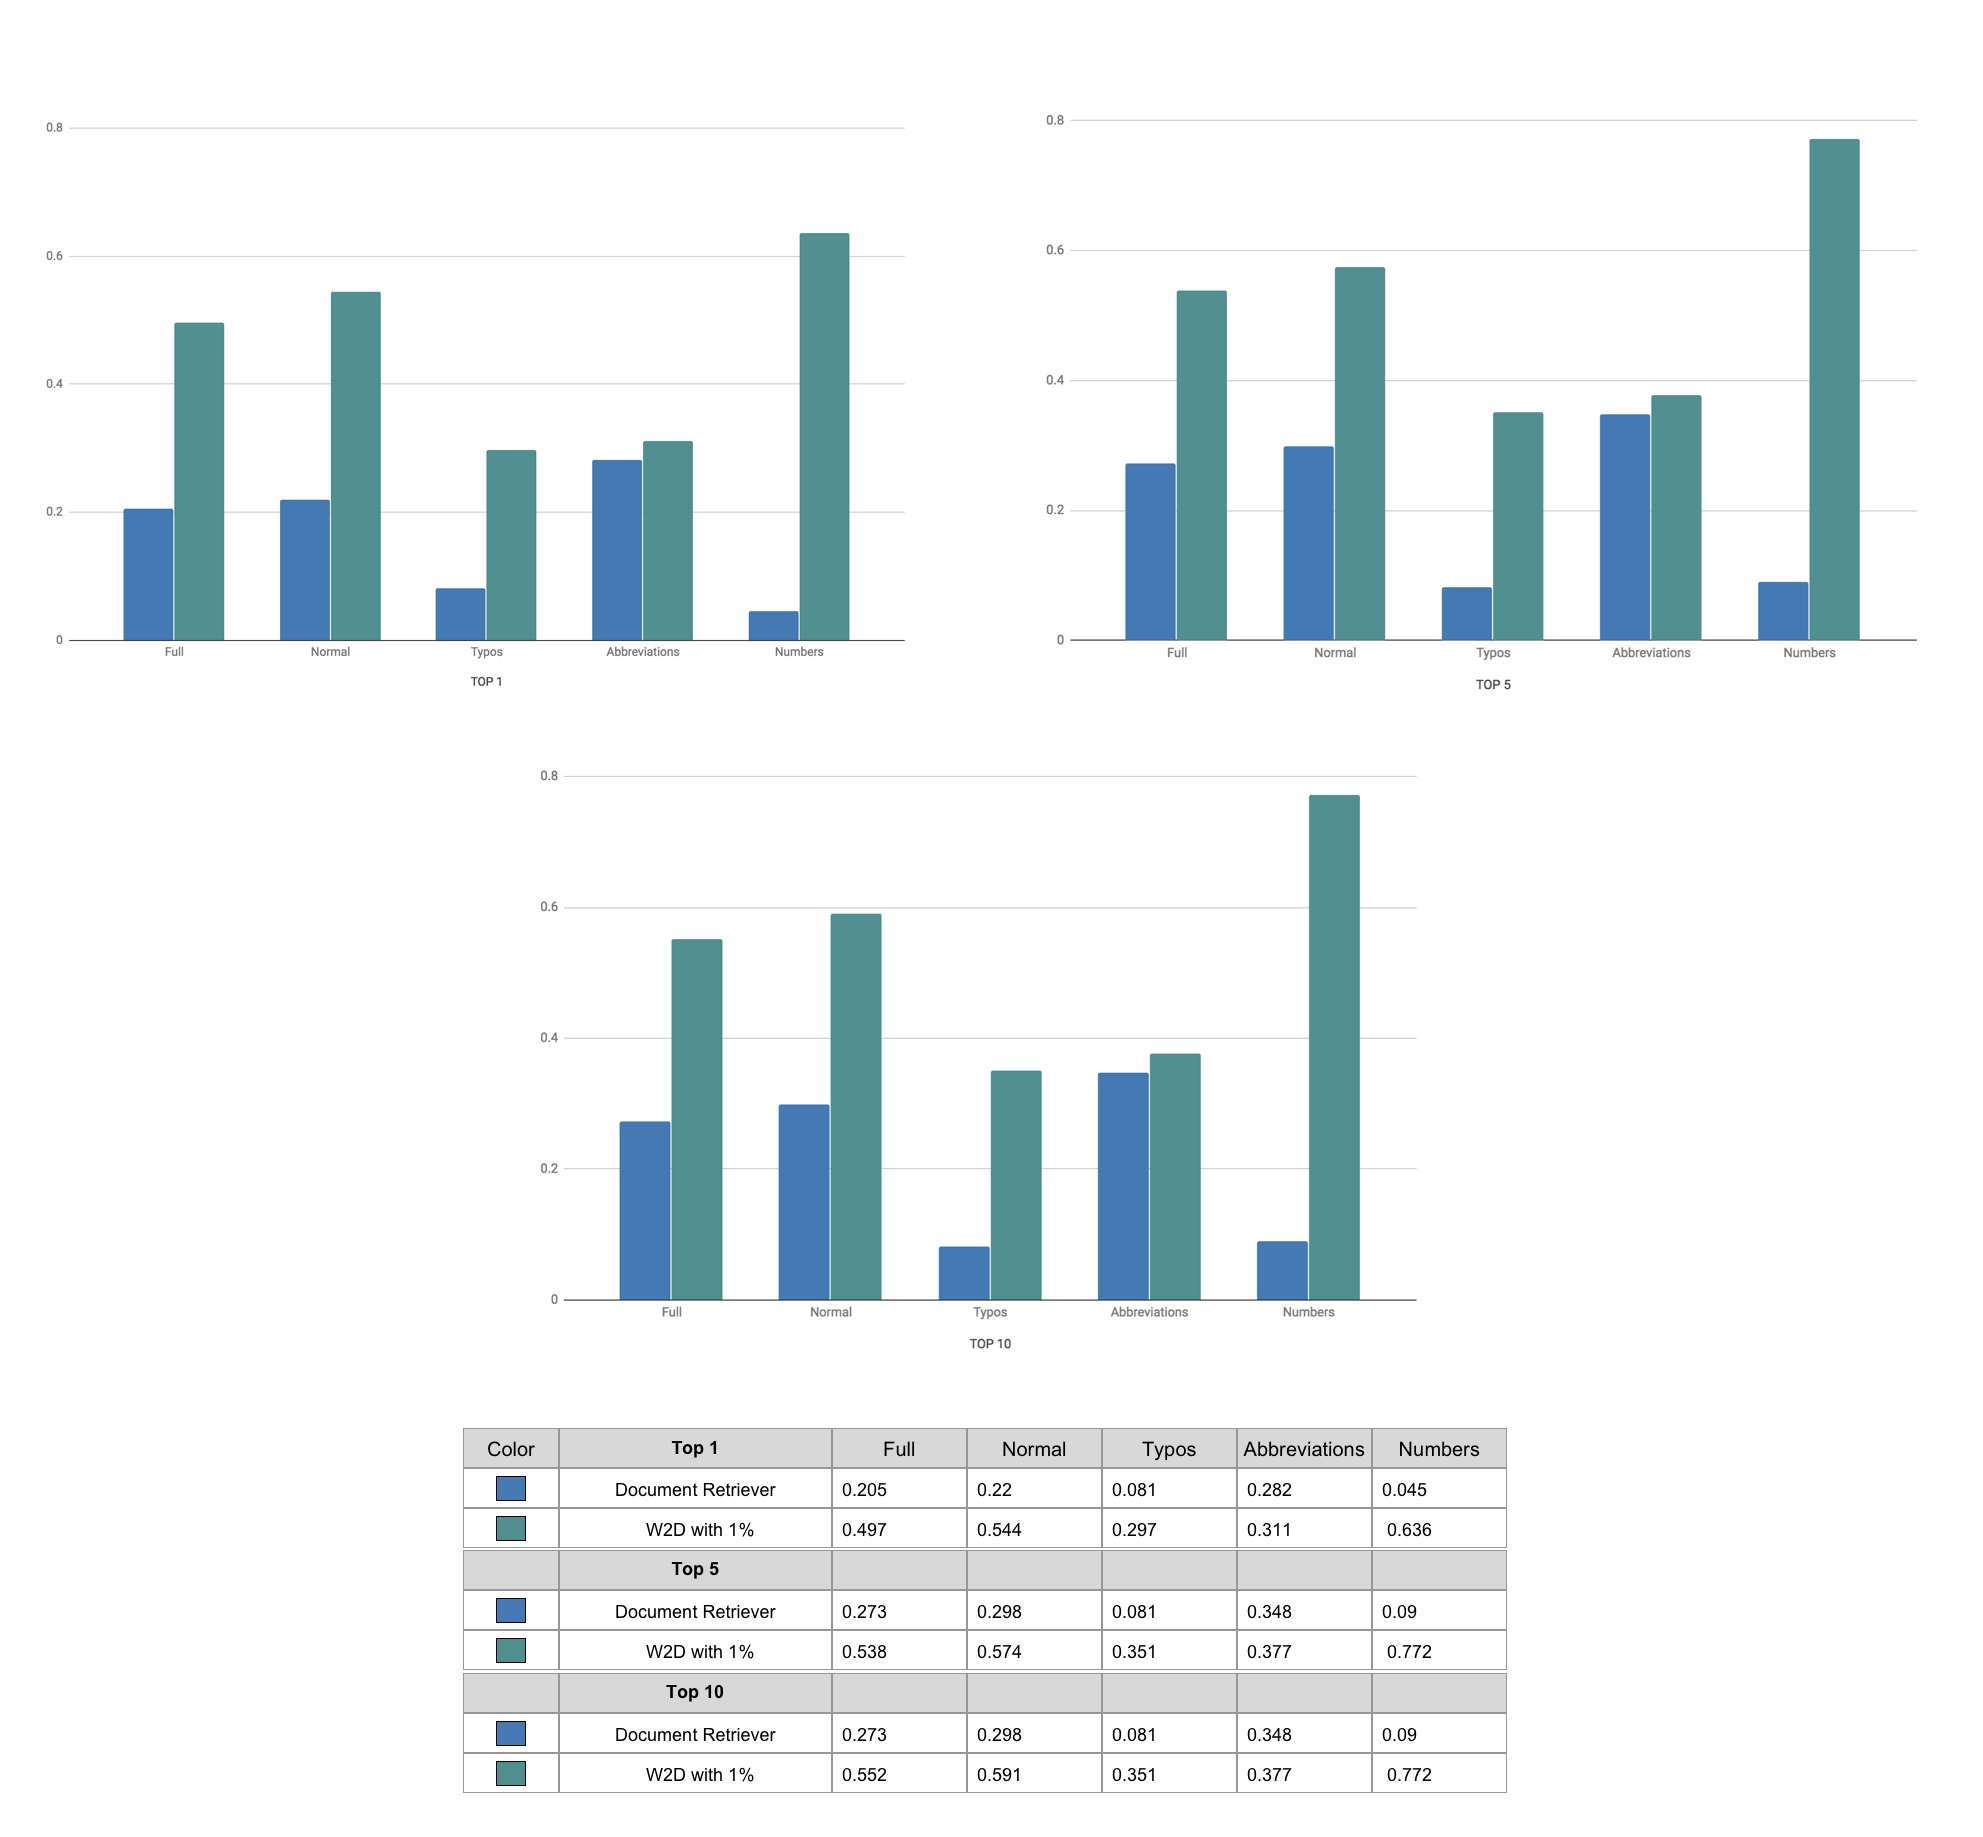
\includegraphics[scale=0.23]{w2d-results-acc-obf.png}
  \end{center}
  \captionsetup{width=.75\linewidth}
  \caption{Facebook's document retriever vs. Word2doc Performance [Accuracy] using all components of the W2D-VD-400 evaluation
  data. Accuracies are evaluated on the top one, top five and top ten retrieved documents.}
  \label{fig:w2d-results-acc-obf}
\end{figure}

Word2doc performs significantly better than Facebook's document retriever when it comes to pure accuracies. On all
components, word2doc outscores the document retriever, most noticeably when it comes to dealing with typos and turning numbers
into their written form and vice-versa. This trend is persistent across the top one, top five and top ten graphs. In fact there
does not seem to be much of a difference in the shapes of the three graphs. While the overall accuracies increase as the
number of retrieved documents increases, the ratio between accuracies seems to largely stay the same. It is interesting to note that
accuracies between the top five and the top ten retrieved documents do not change at all when it comes to the document retriever.

It is not surprising to see, that the "normal" component scored the highest (except for the "numbers" component) as the other
components perform worse and thus negatively impact the entire dataset. However, it is strange that the numbers component scored
so high. I explain this largely through the fact that there are only 22 data points in the numbers components, simply too few
to report a representative result. Perhaps there were also enough relevant words in the query that helped word2doc find the
correct document. For example, if the query was "King Henry the fifth", perhaps it had enough information in "King Henry" that it
could identify the correct King Henry (assuming the previous four kings are not in the dataset).

Overall, word2doc seems to be decently robust towards more complicated queries. It has the most difficulty with typos, which
is not surprising. However, it still has less difficulty with typos than the document retriever. It is surprising to see that
the document retriever performs better on abbreviations than on the complete test set or even just the "normal" component.

\section{Performance measured through MAP}
\label{results:map}

Word2doc and Facebook's document retriever can both return a list of ranked retrieval results. To measure the quality of these
results, I use mean average precision on the top five retrieved documents, as explained in section \ref{exp:map}. I only calculated
MAP scores on one of the ten 1\% samples.\footnote{Deciding by hand if 2000 documents are relevant to a query is a lot of work, and I did not
want to evaluate 20,000 documents by hand.} The
results presented in Figure \ref{fig:w2d-results-map} are thus not averaged across multiple samples but are only based on a single
sample. All MAP scores are computed using the W2D-VD-400 test-set as evaluation data. Furthermore, to better understand the MAP
score of the full W2D-VD-400 dataset, I also calculated MAP scores on all of its sub-components just like in the section above.

\begin{figure}
  \begin{center}
    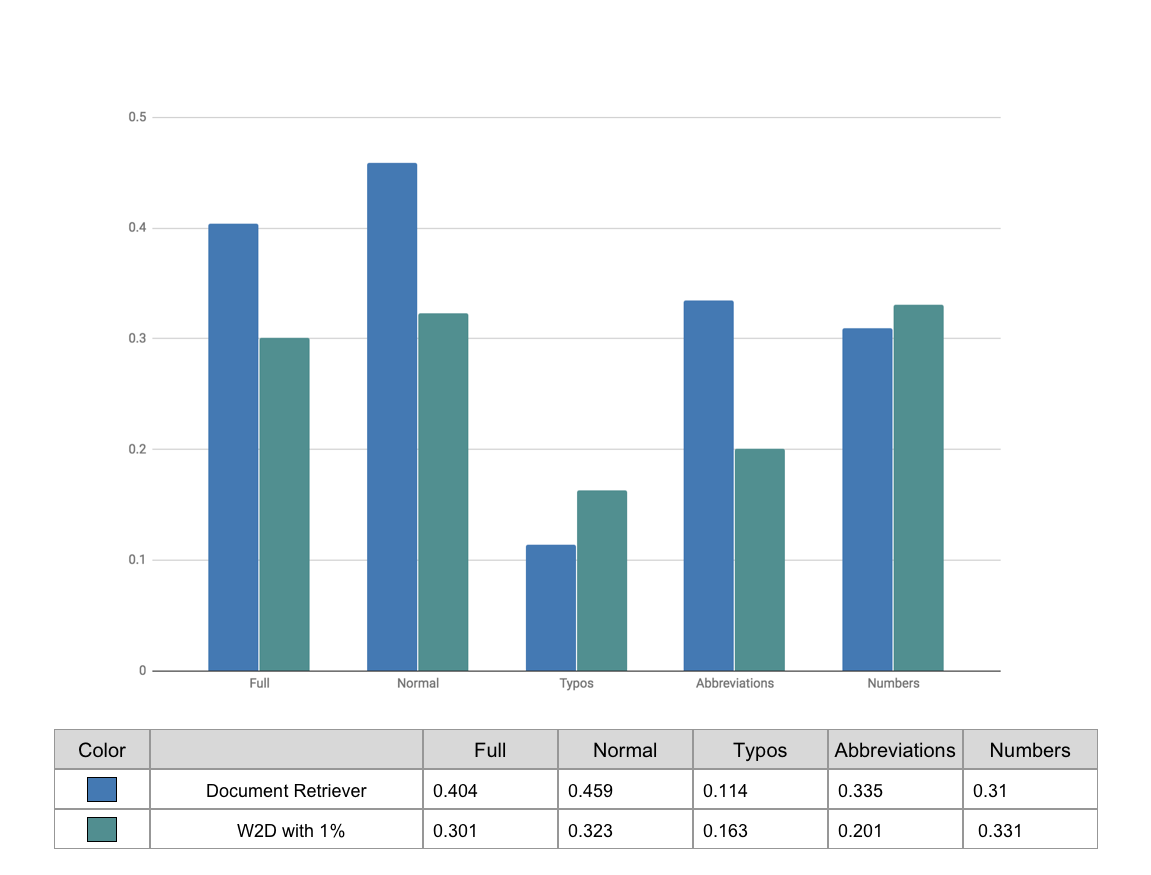
\includegraphics[scale=0.28]{w2d-results-map.png}
  \end{center}
  \captionsetup{width=.75\linewidth}
  \caption{Facebook's document retriever vs. Word2doc Performance [MAP] with the full W2D-VD-400 used as evaluation data on the
  top five retrieved documents.}
  \label{fig:w2d-results-map}
\end{figure}

Looking at Figure \ref{fig:w2d-results-map}, it becomes apparent that the document retriever performs better than word2doc. While
creating the MAP scores, I noticed that word2doc only rarely returned other documents within the retrieved set of documents that were also
relevant, assuming it did find the target document. In fact word2doc is very bad at predicting five or ten documents
that are all relevant.

The document retriever performed much better in general. However, it severely lacks understanding of context.
This makes sense since it is purely based on statistics. The few cases in which word2doc did return relevant documents (besides
the target) were cases in which the other documents contextually and semantically made sense. This suggests that word2doc is able
to group document's together based on their semantical similarity, at least to a certain degree. The fact that word2doc can only
choose from 1\% of all Wikipedia documents, whereas Facebook's document retriever can retrieve documents from the entire
English Wikipedia corpus probably had a large impact on performance. My guess is that many documents that the document retriever
found could not be found by
word2doc because they were simply not included in the training data. Furthermore, word2doc trains on accuracy, not MAP scores.
Thus, it is also possible that word2doc optimizes only to find the target document and not to yield logits which reflect a ranking
in the documents. Hence, it might help to optimize for another metric than accuracy. MAP is not an option however, unless word2doc is
trained on a dataset for which there is a golden standard so that MAP scores can be calculated automatically.

It should also be noted that word2doc's MAP scores were significantly improved by its base accuracies. Word2doc's accuracies are
a lot higher compared to those of the document retriever. While the document retriever gets its MAP score from more or less all
documents in the ranking, word2doc mostly gets its score by predicting the first document correctly much more often than the
document retriever. Since higher ranked documents are weighted more heavily than lower ranked documents, predicting the first
document correctly makes a big difference in the final MAP score.

Looking at the impact of individual components that make up W2D-VD-400, it is not surprising to see that the typos, abbreviations
and numbers had a negative impact on the overall score. The test data component without any obfuscation (the "normal" component)
performed better than the entire dataset combined. Except for the typos component, the individual components did not perform
that much worse, suggesting that both systems can
yield results that are somewhat relevant despite data obfuscation. Furthermore, it is interesting that the
spread in the graphs for word2doc's scores is less than that of the document retriever. This suggests that word2doc is overall more
robust towards obfuscated queries than the document retriever, which is good.

It is also interesting to compare the accuracies on the top five documents retrieved from Figure \ref{fig:w2d-results-acc-obf} and
compare them to their MAP scores. Word2doc's graphs have a similar shape, but those of the document retriever do not. The numbers
component has a relatively high MAP score, but a very low accuracy. This suggests that the document retriever is able to
retrieve documents that are relevant to the query, but it is unable to retrieve the target document.

One should not forget that in order to get reliable MAP scores, large and diverse test sets are required. That is
hardly the case for the typo component (size 37), abbreviation component (size 46) and number component (size 22).
Thus, these calculated MAP scores are subjective to a certain degree and should be treated with care.

